\documentclass[envcountsect,dvips]{beamer}

\setbeamertemplate{background canvas}[vertical shading][bottom=yellow!20,top=blue!10]
%\usetheme{Darmstadt}
\usetheme{Warsaw}
%\usefonttheme[onlysmall]{structurebold}

\usepackage{natbib}
\usepackage{bibentry}
\bibliographystyle{apalike}
\usepackage{chngcntr}

\usepackage[utf8]{inputenc}
\usepackage{default}
\usepackage{amsmath}
\usepackage{amsfonts}
\usepackage{amssymb}

\usepackage{color,xcolor,ucs}% para textcolor
\begin{document}

%%%%%%%%%%%%%%%%%%%%%%%%%%%%%%%%%%%%%%%%%%%%%%%%%%%%%%%%%%%%%%%%%%%%%%%%%%%%%%%%
%%%%%%%%%%%%%%%%%%%%%%%%%%%%%%%%%%%%%%%%%%%%%%%%%%%%%%%%%%%%%%%%%%%%%%%%%%%%%%%%
\section{Filtering using a FIR}
%%%%%%%%%%%%%%%%%%%%%%%%%%%%%%%%%%%%%%%%%%%%%%%%%%%%%%%%%%%%%%%%%%%%%%%%%%%%%%%%
\begin{frame}{Filtering  system}
\begin{block}{Impulse response}
\tiny
\begin{equation}
\begin{matrix}
h[n] & = & h_0 \delta[n] &+& h_1\delta[n-1] &+& h_2\delta[n-2] &... &+& h_M \delta[n-M]\\
H(Z) & = & h_0           &+& h_1Z^{-1}      &+& h_2 Z^{-2}     &... &+& h_M Z^{-M} 
\end{matrix}
\end{equation}
\normalsize
\end{block}
\begin{figure}[!htb]
\centering
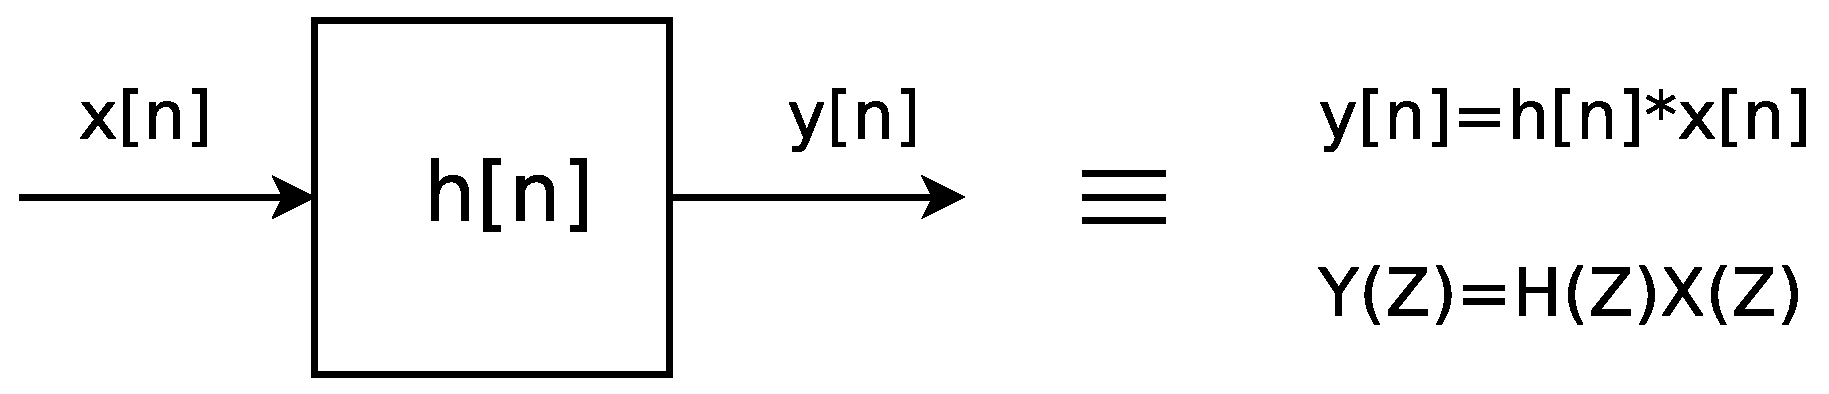
\includegraphics[width=6cm]{images/system.eps}
\caption{Filtering  system}
\label{fig:system}
\end{figure} 
\end{frame}
%%%%%%%%%%%%%%%%%%%%%%%%%%%%%%%%%%%%%%%%%%%%%%%%%%%%%%%%%%%%%%%%%%%%%%%%%%%%%%%%
\begin{frame}{Filtering  system}
\begin{block}{Impulse response}
\tiny
\begin{equation}
\begin{matrix}
h[n] & = & h_0 \delta[n] &+& h_1\delta[n-1] &+& h_2\delta[n-2] &... &+& h_M \delta[n-M]\\
H(Z) & = & h_0           &+& h_1Z^{-1}      &+& h_2 Z^{-2}     &... &+& h_M Z^{-M} 
\end{matrix}
\end{equation}
\normalsize
\end{block}
\begin{figure}[!htb]
\centering
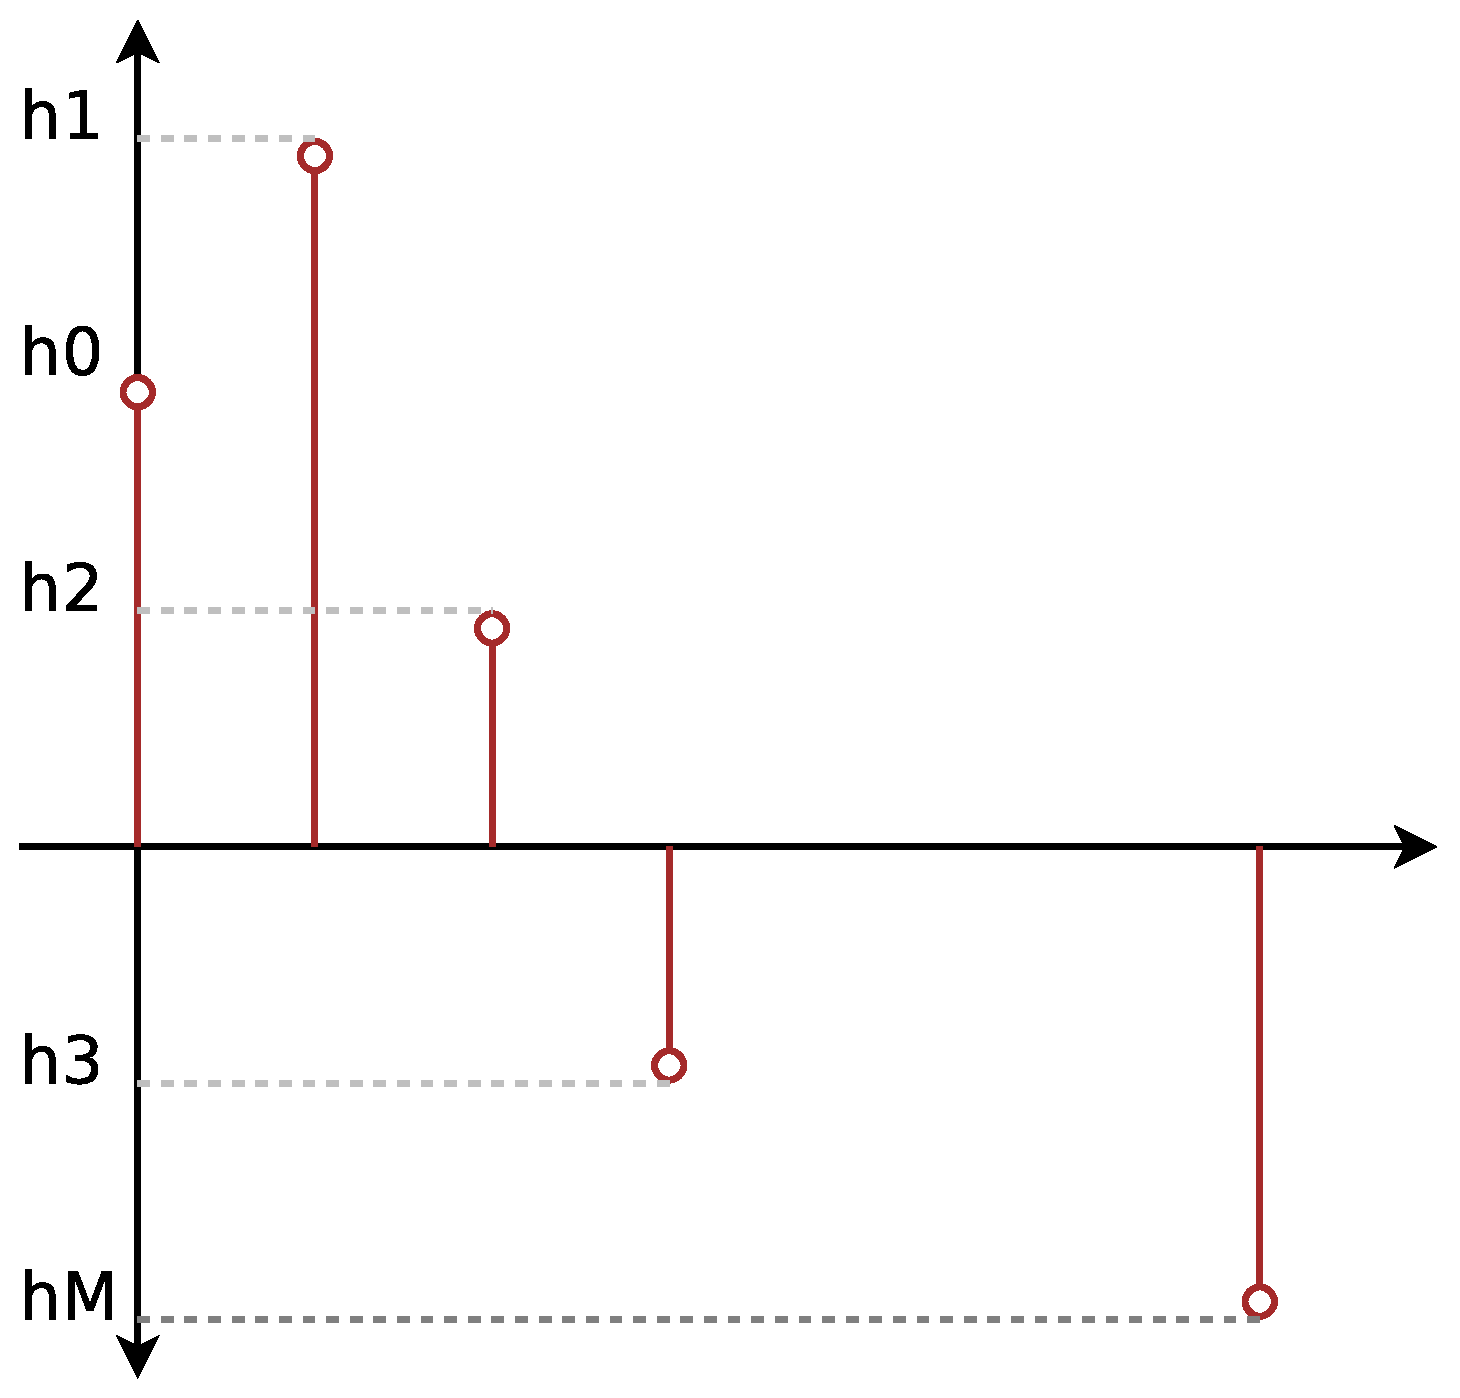
\includegraphics[width=4cm]{images/response.eps}
\caption{h[n] Impulse response}
\label{fig:system}
\end{figure} 
\end{frame}
%%%%%%%%%%%%%%%%%%%%%%%%%%%%%%%%%%%%%%%%%%%%%%%%%%%%%%%%%%%%%%%%%%%%%%%%%%%%%%%%
%%%%%%%%%%%%%%%%%%%%%%%%%%%%%%%%%%%%%%%%%%%%%%%%%%%%%%%%%%%%%%%%%%%%%%%%%%%%%%%%
\section{Fourier transform of sinc function}
%%%%%%%%%%%%%%%%%%%%%%%%%%%%%%%%%%%%%%%%%%%%%%%%%%%%%%%%%%%%%%%%%%%%%%%%%%%%%%%%
\begin{frame}{Knowing the Fourier transform of $h_a[n]$}
\begin{block}{Impulse response}
\tiny
\begin{equation}
\begin{matrix}
h_a[n] & = & h_0 \delta[n] &+& h_1\delta[n-1] &+& h_2\delta[n-2] &... &+& h_M \delta[n-M]\\
H_a(Z) & = & h_0           &+& h_1Z^{-1}      &+& h_2 Z^{-2}     &... &+& h_M Z^{-M} 
\end{matrix}
\end{equation}
\normalsize
\end{block}
\begin{block}{Z transform $\xrightarrow{ Z=e^{jw} }$ Fourier transform}
\begin{equation}
H_a(Z)  \xrightarrow{ Z=e^{jw} } H_a(e^{jw}) 
\end{equation}
\end{block}


\begin{equation}
 h_a[n]=\begin{cases}
 \frac{sin(\pi~a~n)}{\pi~n} & \text{ if } n \neq 0 \\ 
 a & \text{ if } n = 0
\end{cases}
\end{equation}

\begin{equation}
 H_a(e^{jw})=\begin{cases}
 1 & \text{ if } W \leq a \pi \\ 
 0 & \text{ if } W >    a \pi
\end{cases}
\end{equation}

\end{frame}

%%%%%%%%%%%%%%%%%%%%%%%%%%%%%%%%%%%%%%%%%%%%%%%%%%%%%%%%%%%%%%%%%%%%%%%%%%%%%%%%
\begin{frame}{Knowing the Fourier transform of $h_a[n]$}
\begin{block}{Function $h_a[n]$}
\begin{figure}[!htb]
\centering
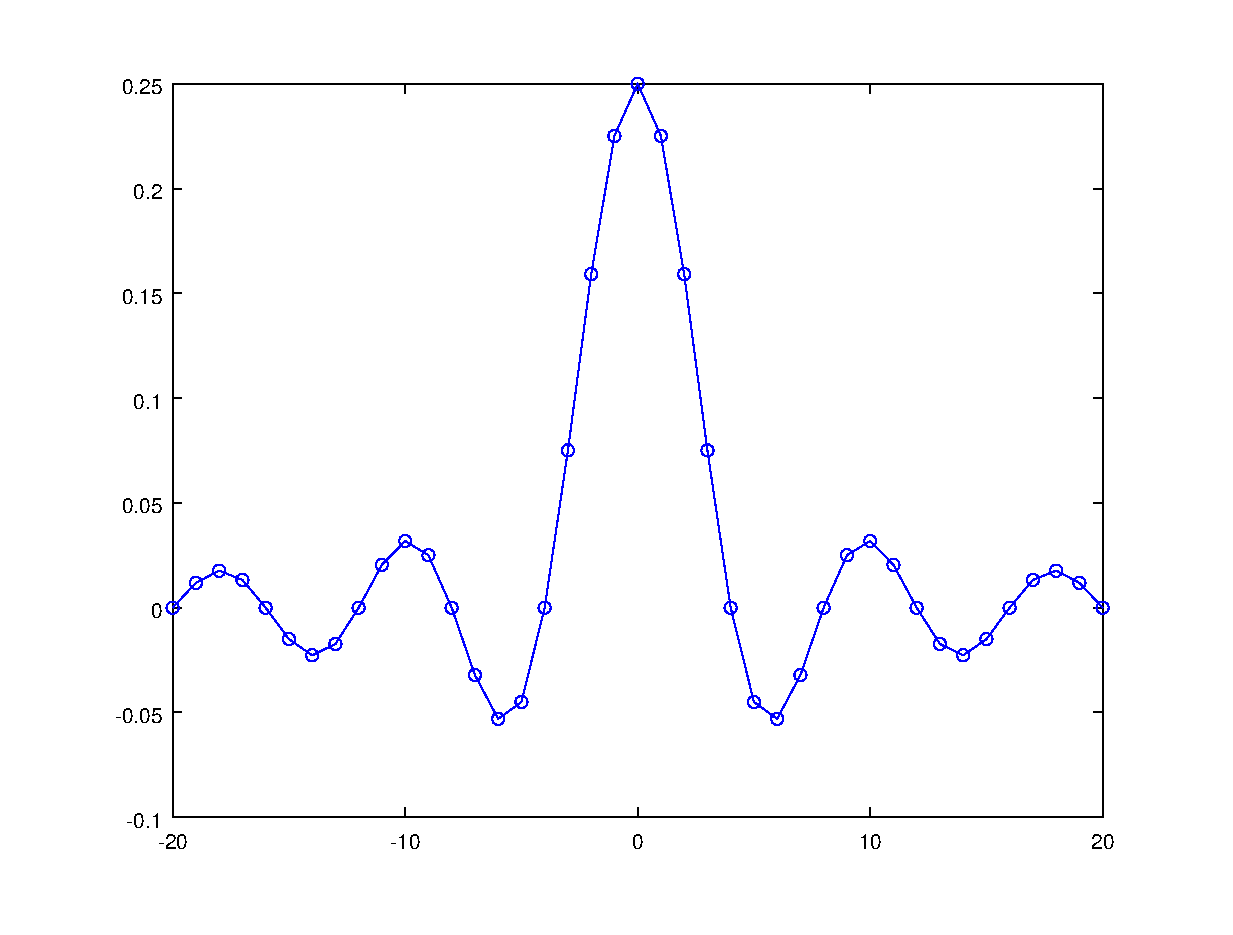
\includegraphics[width=6cm]{images/xn.eps}
\caption{$h_a[n]$ with $a=0.25$ and 41 points}
\label{fig:xn}
\end{figure}  
\end{block}
\end{frame}

%%%%%%%%%%%%%%%%%%%%%%%%%%%%%%%%%%%%%%%%%%%%%%%%%%%%%%%%%%%%%%%%%%%%%%%%%%%%%%%%
\begin{frame}{Knowing the Fourier transform of $h_a[n]$}
\begin{block}{Fourier transform of $h_a[n]$}
\begin{figure}[!htb]
\centering
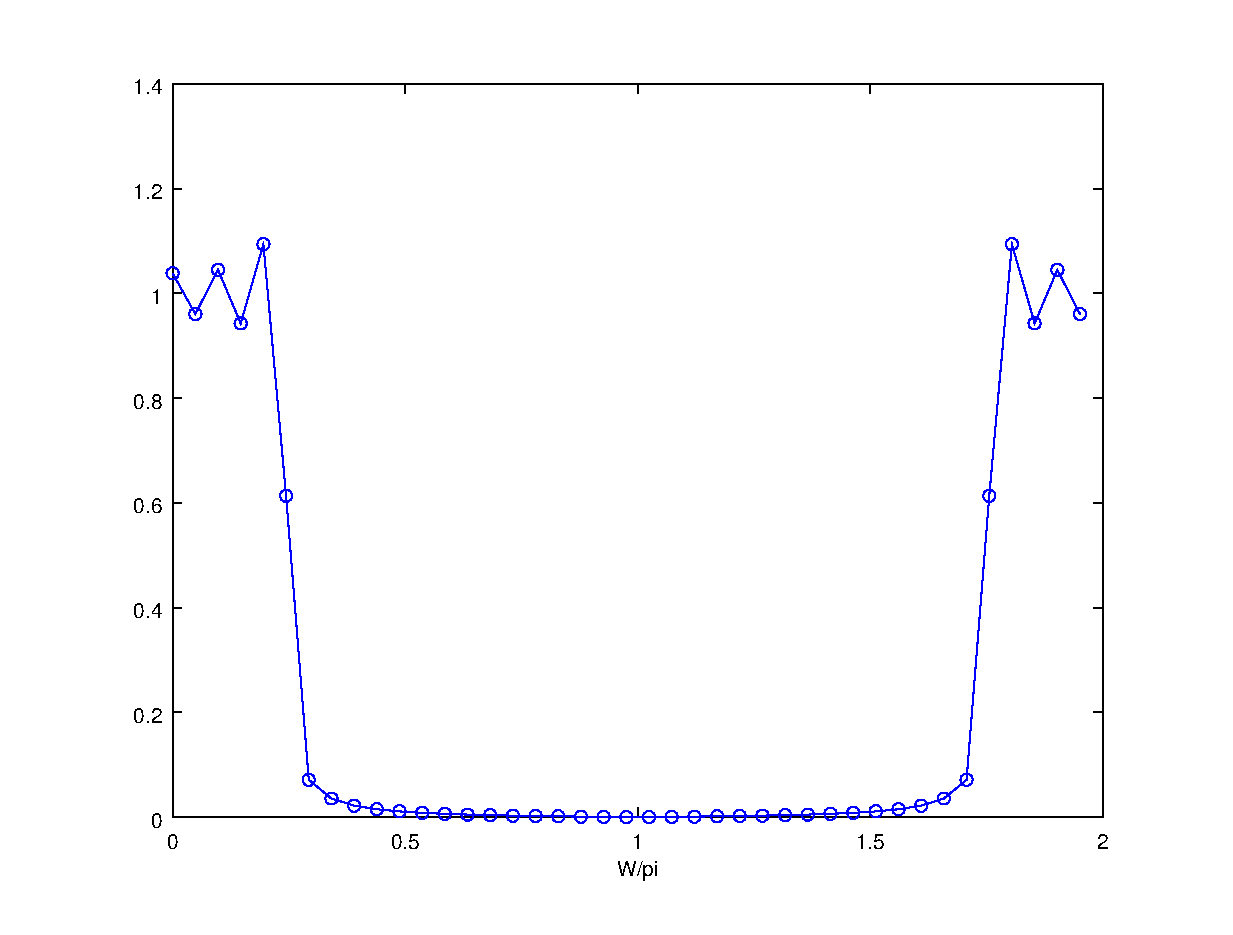
\includegraphics[width=6cm]{images/XW.eps}
\caption{$H_a(W)$ with $a=0.25$ and 41 points}
\label{fig:XW}
\end{figure}  
\end{block}
\end{frame}

%%%%%%%%%%%%%%%%%%%%%%%%%%%%%%%%%%%%%%%%%%%%%%%%%%%%%%%%%%%%%%%%%%%%%%%%%%%%%%%%
\begin{frame}{Knowing the Fourier transform of $h_a[n]$}
\begin{block}{Fourier transform of $h_a[n]$}
\begin{figure}[!htb]
\centering
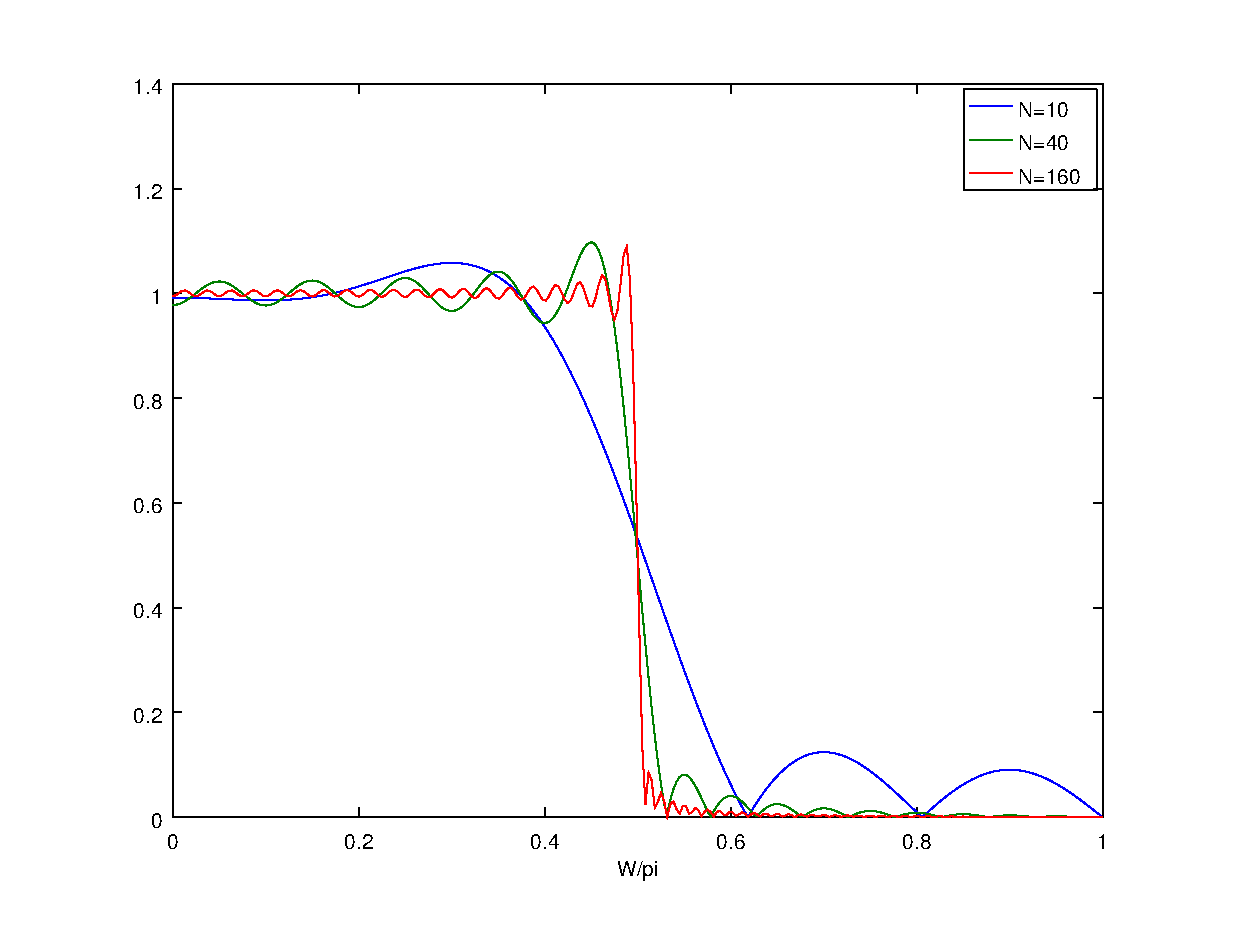
\includegraphics[width=6cm]{images/XW5.eps}
\caption{$H_a(W)$ with $a=0.5$}
\label{fig:XW5}
\end{figure}  
\end{block}
\end{frame}

%%%%%%%%%%%%%%%%%%%%%%%%%%%%%%%%%%%%%%%%%%%%%%%%%%%%%%%%%%%%%%%%%%%%%%%%%%%%%%%%
%%%%%%%%%%%%%%%%%%%%%%%%%%%%%%%%%%%%%%%%%%%%%%%%%%%%%%%%%%%%%%%%%%%%%%%%%%%%%%%%
\section{Efecto do janelamento}
%%%%%%%%%%%%%%%%%%%%%%%%%%%%%%%%%%%%%%%%%%%%%%%%%%%%%%%%%%%%%%%%%%%%%%%%%%%%%%%%
\begin{frame}{Janelamento da função sinc}
\begin{block}{Janela de Hanning de $N=61$ amostras}
 \begin{equation}
  hanning[n]=0.5(1-cos(\frac{2 \pi n }{N-1}))
 \end{equation}
\end{block}
\begin{figure}[!htb]
\centering
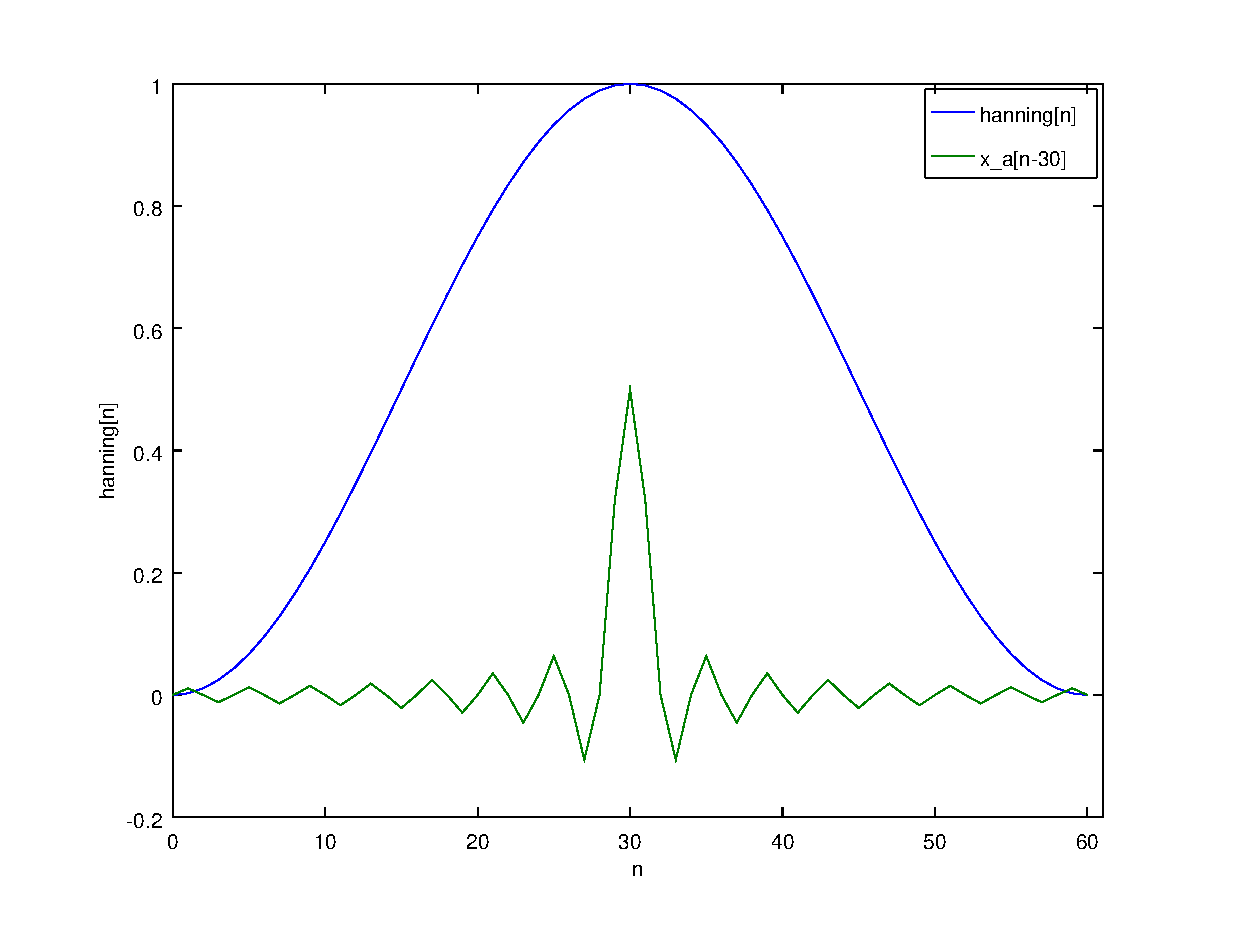
\includegraphics[width=5cm]{images/hanning.eps}
\caption{Hanning window and $h_a[n-30]$ for $a=0.5$}
\label{fig:hanningn}
\end{figure}  
\end{frame}

%%%%%%%%%%%%%%%%%%%%%%%%%%%%%%%%%%%%%%%%%%%%%%%%%%%%%%%%%%%%%%%%%%%%%%%%%%%%%%%%
\begin{frame}{Janelamento da função sinc}
\begin{block}{Fourier transform  de uma janela de Hanning de $N=61$ amostras}
 \begin{equation}
  HANNING(W)=FFT\{hanning[n]\}
 \end{equation}
\end{block}
\begin{figure}[!htb]
\centering
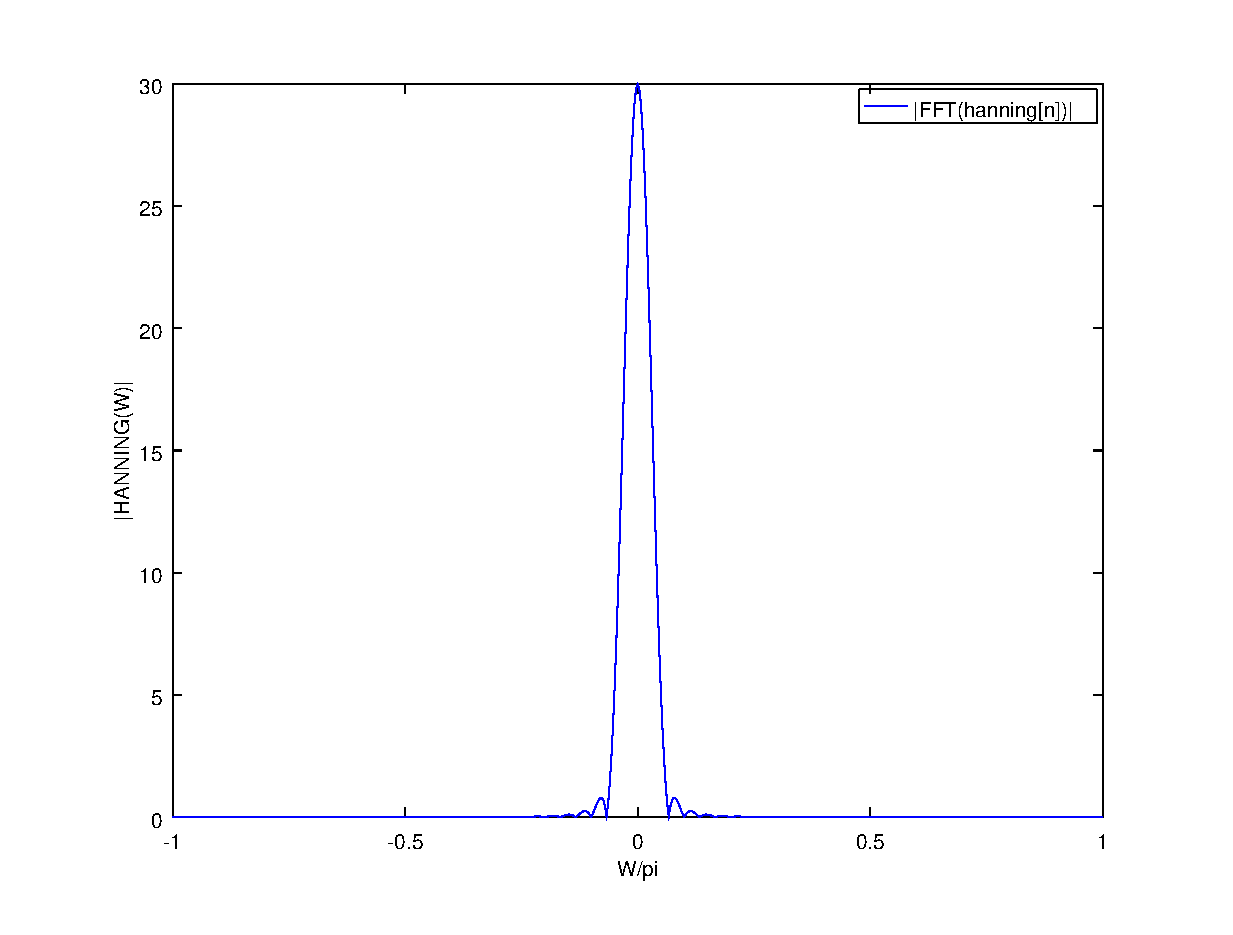
\includegraphics[width=5cm]{images/hanningfft.eps}
\caption{Fourier transform of Hanning window}
\label{fig:hanningw}
\end{figure}  
\end{frame}

%%%%%%%%%%%%%%%%%%%%%%%%%%%%%%%%%%%%%%%%%%%%%%%%%%%%%%%%%%%%%%%%%%%%%%%%%%%%%%%%
\begin{frame}{Conhecendo que a transformada de fourier de $h_a[n]~hanning[n+D]$}
\begin{block}{Fourier transform of $h_a[n]~hanning[n+D]$}
 \begin{equation}
  H_a(W)*hanning(W) \equiv convolution\{H_a(W),hanning(W)\}
 \end{equation}
\end{block}
\begin{figure}[!htb]
\centering
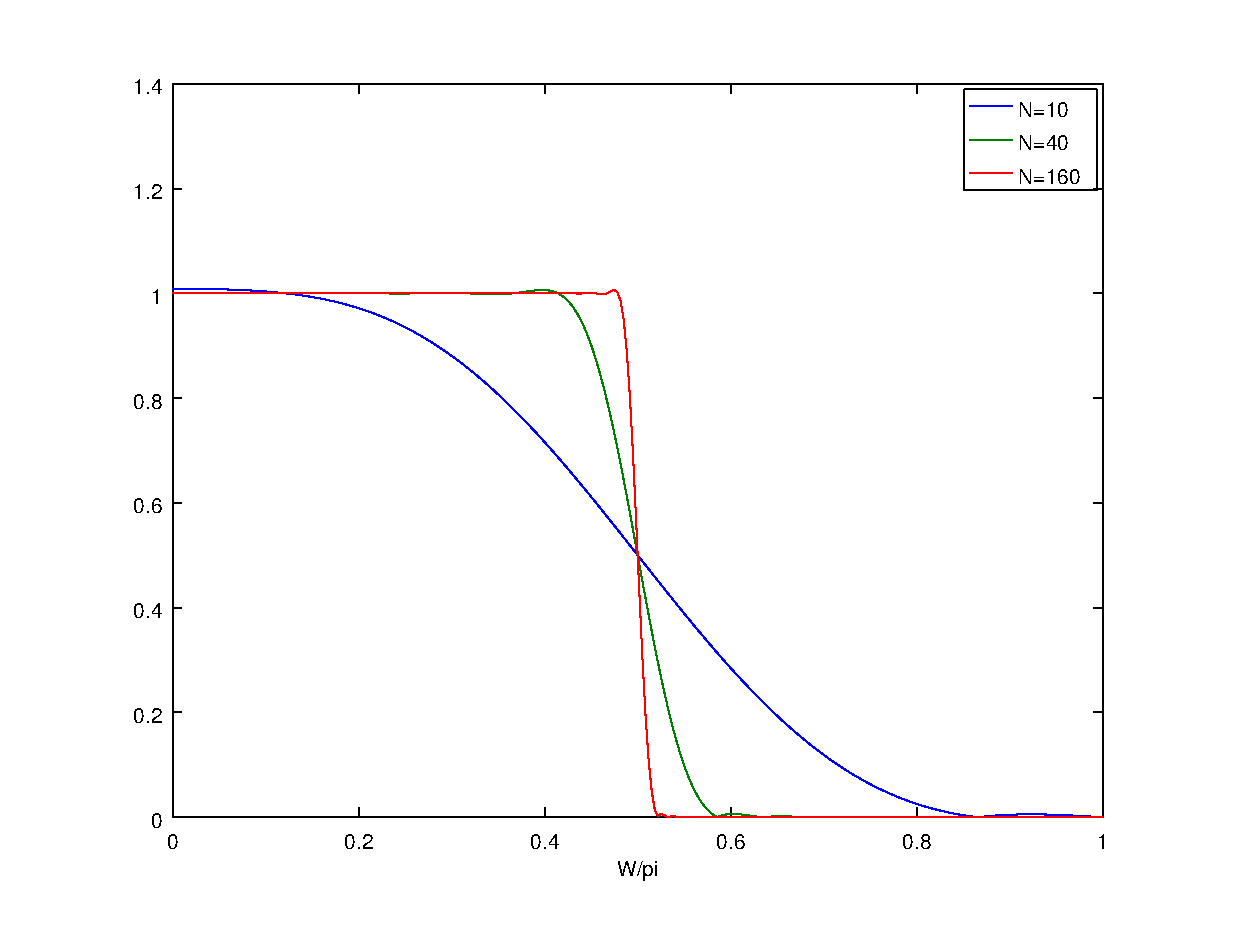
\includegraphics[width=5cm]{images/XW5h.eps}
\caption{$H_a(W)*hanning(W)$ para $a=0.5$}
\label{fig:XW5h}
\end{figure}  
\end{frame}


%%%%%%%%%%%%%%%%%%%%%%%%%%%%%%%%%%%%%%%%%%%%%%%%%%%%%%%%%%%%%%%%%%%%%%%%%%%%%%%%
\begin{frame}{Tipos de janelas }

\begin{block}{Hanning}
 \begin{equation}
  hanning[n]=0.5(1-cos(\frac{2 \pi n }{N-1}))
 \end{equation}
\end{block}
 
\begin{block}{Hamming}
 \begin{equation}
  hamming[n]= \alpha - \beta\ \cos\left( \frac{2 \pi n}{N - 1} \right), \alpha+\beta=1
 \end{equation}
\end{block}

\begin{block}{Blackman}
\begin{equation}
    w(n)=a_0 - a_1 \cos \left ( \frac{2 \pi n}{N-1} \right) + a_2 \cos \left ( \frac{4 \pi n}{N-1} \right)
\end{equation}
\begin{equation}
    a_0=\frac{1-\alpha}{2};\quad a_1=\frac{1}{2};\quad a_2=\frac{\alpha}{2}\, 
\end{equation}
\end{block}

\end{frame}


%%%%%%%%%%%%%%%%%%%%%%%%%%%%%%%%%%%%%%%%%%%%%%%%%%%%%%%%%%%%%%%%%%%%%%%%%%%%%%%%
%%%%%%%%%%%%%%%%%%%%%%%%%%%%%%%%%%%%%%%%%%%%%%%%%%%%%%%%%%%%%%%%%%%%%%%%%%%%%%%%
\section{FIR low pass to }

\begin{block}{FIR Low-pass filter with cut-off at $a\pi$ (normalized to $2\pi$)}
\tiny
 \begin{equation}
 \begin{matrix}
h_a[n] & = & h_0 \delta[n] &+& h_1\delta[n-1] &+& h_2\delta[n-2] &... &+& h_M \delta[n-M]\\
H_a(Z) & = & h_0           &+& h_1Z^{-1}      &+& h_2 Z^{-2}     &... &+& h_M Z^{-M}    
 \end{matrix}
 \end{equation}
\normalsize
\end{block}
\begin{block}{If M is even then: High pass filter with cut-off at $a\pi$}
 \begin{equation}
  Z^{-M/2}-H_a(Z)
 \end{equation}
\end{block}
\begin{block}{High pass filter with cut-off at $(1-a)\pi$}
 \begin{equation}
 H_a(-Z)
 \end{equation}
\end{block}
\begin{block}{Band pass filter with cut-off at $(1-a)\pi$ and $b\pi$}
 \begin{equation}
 H_b(Z)*H_a(-Z)
 \end{equation}
\end{block}
\end{document}
